\section{Results}\label{sec:results}

\subsection{Application Interface and Features}
To drive the localization engine, we implemented a comprehensive software suite consisting of a Command Line Interface (CLI) and an interactive Graphical User Interface (UI). These applications facilitate the end-to-end pipeline, from image ingestion to coordinate projection. Key features include:

\begin{itemize}
    \item \textbf{Model Versatility:} Full support for Similarity (4-DOF), Affine (6-DOF), and Projective (8-DOF) transformation models.
    \item \textbf{Algorithmic Tuning:} Real-time configuration of SIFT feature limits, Lowe's ratio, and adaptive RANSAC parameters (epsilon, confidence).
    \item \textbf{Rich Visualization:} Dynamic rendering of keypoint correspondences and projected UAV bounding boxes on the reference map.
    \item \textbf{Artifact Exporting:} Standardized reporting via JSON summaries and ZIP archives for batch processing.
\end{itemize}

\begin{figure}[H]
    \centering
    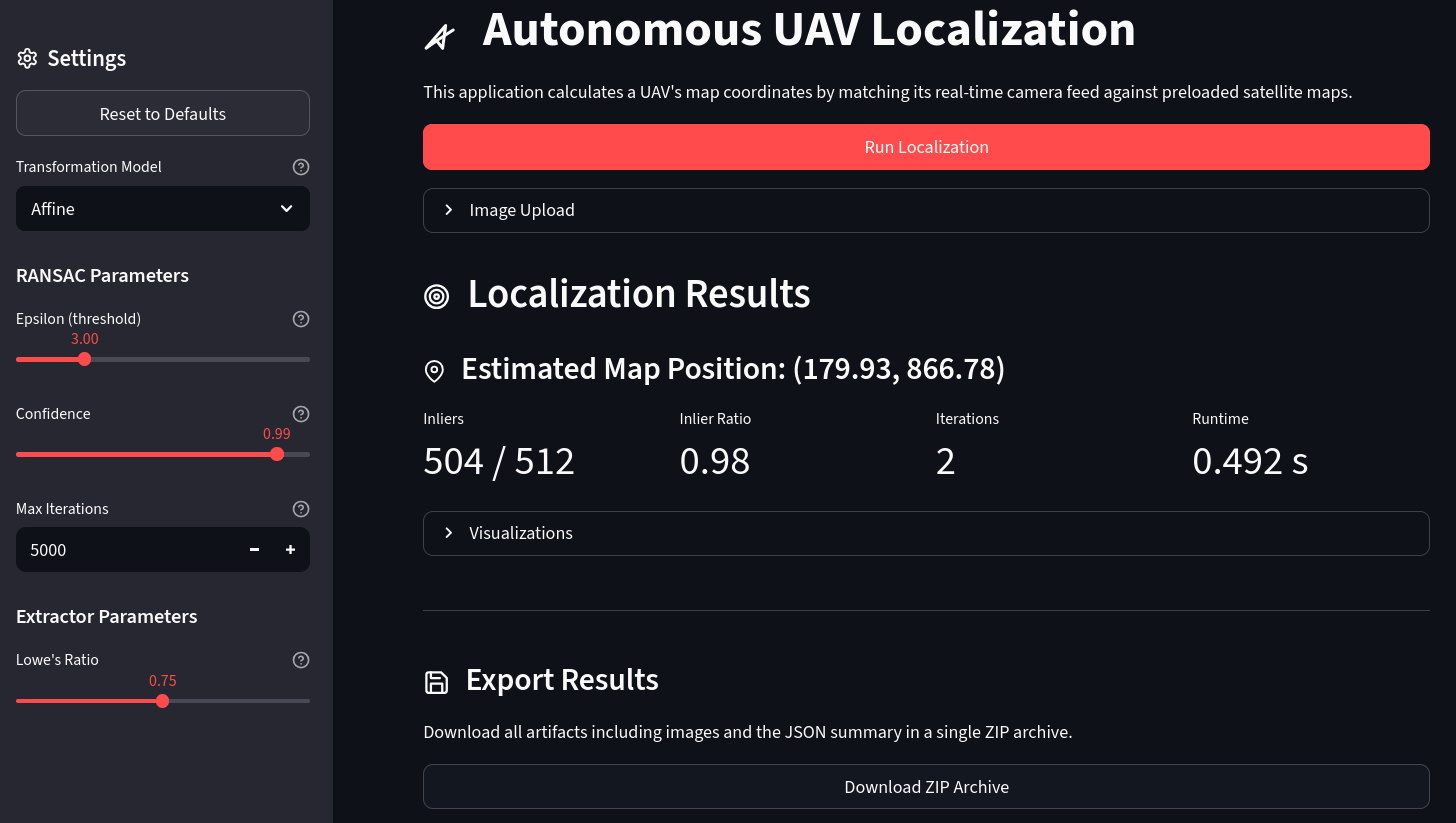
\includegraphics[width=1\columnwidth]{figs/app_ui.png}
    \caption{User Interface for the UAV Localization Application showing successful localization on a synthetic sample.}
    \label{fig:app_ui}
\end{figure}

\subsection{Single Image Match}\label{subsec:single_image_match}
Initial verification was conducted using a single simulated UAV frame. Using an Affine transformation model, the pipeline successfully matched 471 inliers from 478 raw matches ($98.5\%$ inlier ratio). The UAV center was estimated at $(179.99, 866.84)$ pixels in approximately $1.045$ seconds. Visual validation of the correspondences (\autoref{fig:matches_after_ransac}) and the final bounding box (\autoref{fig:map_with_bbox}) confirmed the mathematical correctness of the pipeline under ideal, noise-free conditions.

\begin{figure}[H]
    \centering
    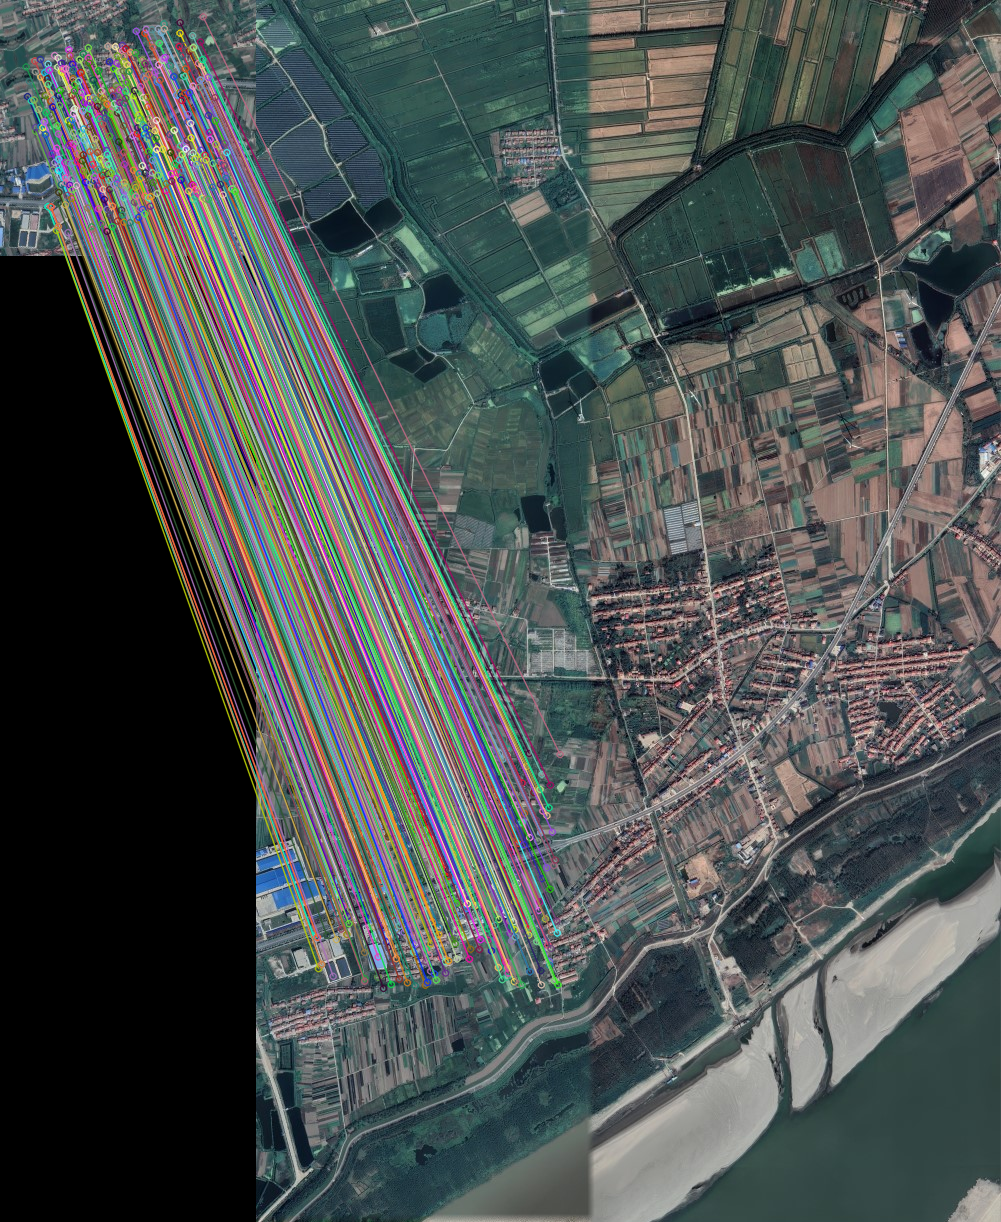
\includegraphics[width=1\columnwidth]{figs/matches_after_ransac.png}
    \caption{Geometrically consistent inlier matches retained after RANSAC filtering.}
    \label{fig:matches_after_ransac}
\end{figure}

\begin{figure}[H]
     \centering
     \begin{subfigure}[b]{0.6\columnwidth}
         \centering
         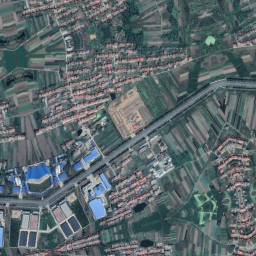
\includegraphics[width=\textwidth]{figs/uav_image.png}
         \caption{Input synthetic UAV frame.}
         \label{fig:uav_frame}
     \end{subfigure}
     \hfill
     \begin{subfigure}[b]{1.0\columnwidth}
         \centering
         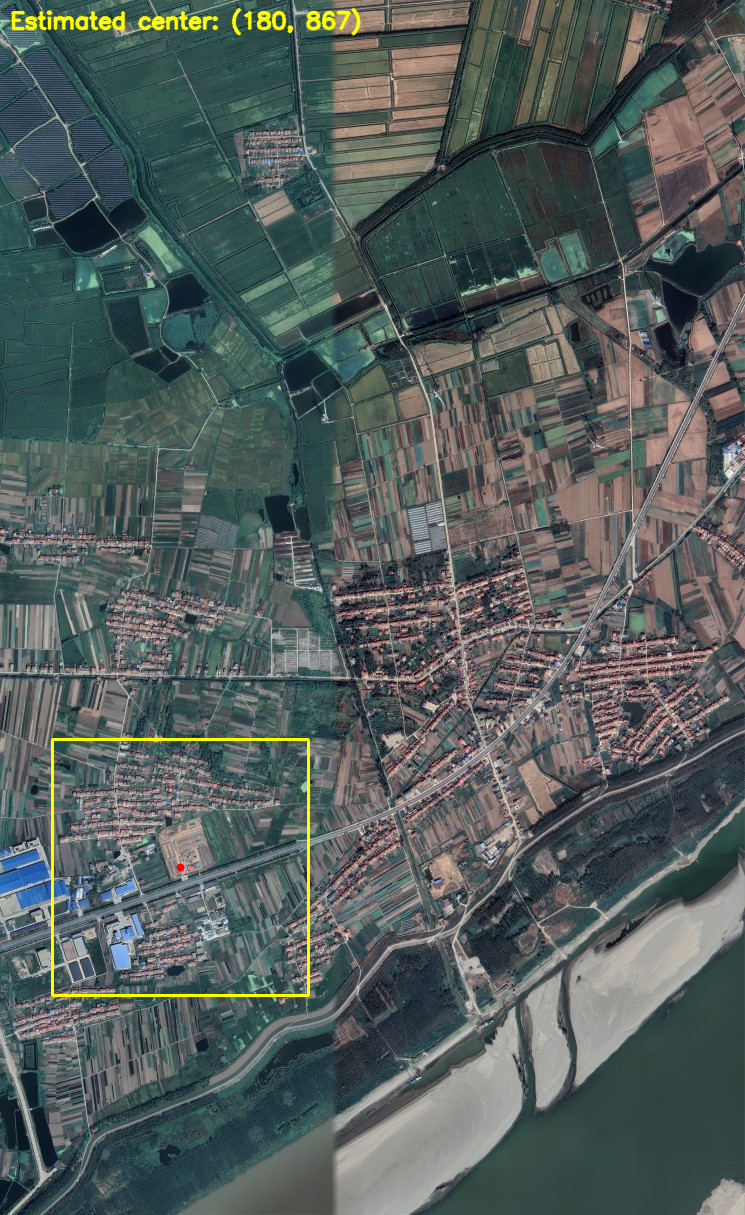
\includegraphics[width=\textwidth]{figs/map_with_estimated_bbox.png}
         \caption{Reference map with the projected UAV footprint.}
         \label{fig:map_footprint}
     \end{subfigure}
        \caption{Single image localization results showing the relationship between the captured frame and the global map.}
        \label{fig:map_with_bbox}
\end{figure}

\subsection{Synthetic Dataset Evaluation}\label{subsec:dataset_evaluation}
We benchmarked the pipeline on a controlled dataset of 60 synthetically deformed satellite crops. The system achieved a $90\%$ technical success rate with a mean RMSE of $16.69$ pixels. The distribution of errors (\autoref{fig:error_distribution}) confirms that the pipeline is highly precise when the UAV image is a direct geometric transformation of the reference map. 

\begin{figure}[H]
    \centering
    
\includegraphics[width=1\columnwidth]{figs/error_distribution.png}
    \caption{Distribution of localization errors across the synthetic dataset.}\label{fig:error_distribution}
\end{figure}

\subsection{Real Dataset Evaluation}\label{subsec:real_evaluation}
The final phase evaluated the pipeline on the UAV-VisLoc dataset \cite{uav_visloc} to compare the Similarity, Affine, and Projective models under real-world conditions. While all models achieved a $84\%$ technical success rate, the accuracy metrics diverged significantly.

\begin{table}[H]
    \caption{Comparative Performance Summary on the UAV-VisLoc Dataset.}\label{tab:real_results}
    \centering
    \begin{tabular}{|l|c|c|c|c|}
        \hline
        \textbf{Model} & \textbf{Success Rate} & \textbf{RMSE (px)} & \textbf{Inlier Ratio} & \textbf{Runtime (s)} \\
        \hline
        Similarity & 84\% & 45,713 & 0.079 & 1.90 \\
        Affine     & 84\% & 146,846 & 0.089 & 1.96 \\
        Projective & 84\% & 15,390 & 0.120 & 2.36 \\
        \hline
    \end{tabular}
\end{table}

\begin{figure}[H]
    \centering
    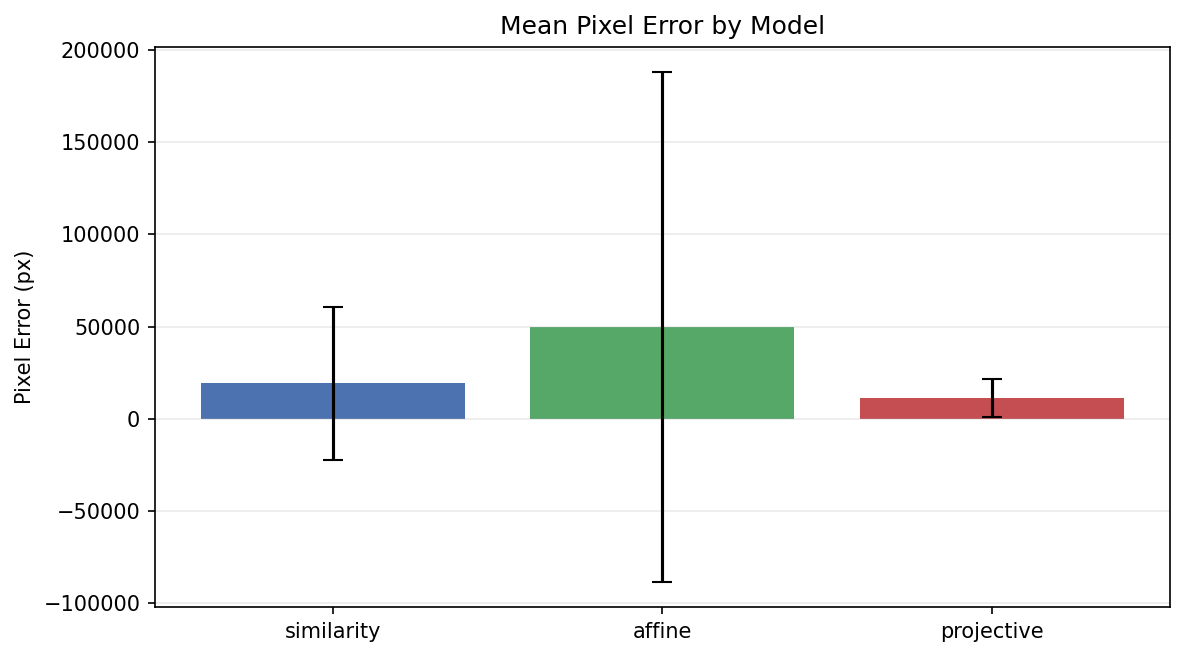
\includegraphics[width=1\columnwidth]{figs/pixel_error_by_model.png}
    \caption{Mean pixel error and standard deviation by transformation model.}
    \label{fig:real_pixel_error}
\end{figure}

The benchmark results (\autoref{tab:real_results}, \autoref{fig:real_pixel_error}) reveal a catastrophic degradation in accuracy compared to the synthetic tests. The Similarity and Affine models exhibited extreme Root Mean Square Errors, whereas the Projective model remained relatively more stable ($15,390$ px). The mean inlier ratio across all models dropped below $0.12$, indicating that over $88\%$ of SIFT correspondences were rejected as outliers. Furthermore, the Projective model exhibited a slightly higher runtime due to the computational overhead of Singular Value Decomposition (SVD) compared to the Normal Equations solver used for the other models.

